\section{Introduction}
\label{sec:introduction}
This note describes the study of  
the invariant mass distribution of jet pairs produced in association 
with a W boson.
The data sample corresponds to an integrated 
luminosity of 5.0 fb${}^{-1}$ collected with the CMS detector at 
$\sqrt{s} = 7$ TeV.

%%%%%%%%%%%%%%%%%%%%%%%%%%%%%%%%%%%%%%%%%%%%%%%
%%%%%%%%%%%%%%%%%%%%%%%%%%%%%%%%%%%%%%%%%%%%%%%
\subsection{Motivation}
\label{sec:motivation}
Recently, the CDF collaboration reported~\cite{cdf_paper} 
the observation of an excess 
of events in  their lepton, missing transverse energy (MET), 
and dijets channel~\cite{cdf_paper,cdf_web} 
(see also the thesis, Ref.~\cite{Cavalierethesis}). 
This excess appears in events with a dijet invariant 
mass in the range of 120-160 GeV, and is consistent with a 
Gaussian distribution centered at $147\pm 4$~GeV. 
The width of the Gaussian distribution is consistent with the dijet mass resolution. 
The excess, observed in 4.3~fb$^{-1}$ of data, consisted of $156\pm42$ events in the electron 
channel and $97\pm38$ in the muon channel, constituting 
a 3.2$\sigma$ deviation from the Standard 
Model prediction~\cite{cdf_paper}. 
An excess was also identified in an inclusive analysis 
of events with a lepton, MET, and two or more jets, 
although with somewhat lower statistical significance. 
More recently, the CDF collaboration extended their 
analysis to 7.3~fb$^{-1}$ of data, finding excesses of 
$240\pm55$ and $158 \pm 45$ events in the electron and 
muon channels, respectively, and resulting in an overall 
significance of 4.1$\sigma$ (assuming a Gaussian shape for 
the signal)~\cite{cdf_web}. 


\par
In view of the possible interpretation as a discovery of physics 
beyond the Standard Model, this anomaly has attracted a lot of attention 
from both experimental and theoretical communities~\cite{BuckleyHooperMartin}. 
If this excess is interpreted as evidence of a new particle 
decaying to a pair of jets, produced in association with a 
leptonically decaying W$^\pm$, then the observed rate requires a 
cross section on the order of $2$--$4$~pb, some 300 times larger 
than is predicted for processes including a Standard Model 
Higgs boson~\cite{BuckleyHooperMartin}.

\par
However, this anomaly has not been confirmed
by a very similar D\O\ analysis~\cite{d0_paper}.
In their analysis of 4.3~fb$^{-1}$ of data, the D\O\ collaboration 
does not report a statistically significant excess consistent with 
that observed by CDF, but does favor (at the $\sim$1$\sigma$ level) 
the presence of a smaller bump-like feature at $\sim$150 GeV, 
corresponding to a production cross section of 
$0.82^{+0.83}_{-0.82}$ pb, about 20\% as large as that reported 
by CDF. The D\O\ collaboration claims to exclude a `bump' arising 
from a 4~pb Higgs-like scalar with a statistical significance 
described by a $p$-value of $8\times 10^{-6}$~\cite{d0_paper}. 

The disagreement between the 
results of CDF and D\O\ are highly unlikely to arise from 
statistical fluctuations, leaving only underlying systematic 
issues or actual new physics as possible 
resolutions~\cite{BuckleyHooperMartin}. Even if 
the CDF excess is not a consequence of new physics, but is rather 
caused by some subtle mismodeling of the Standard Model backgrounds, 
it is possible that this error could propagate to the LHC experiments. 
It is therefore critical that the underlying cause(s) of the 
disagreement between the Tevatron experiments be definitively 
determined. 
Our goal is to repeat the CDF/D\O\ analysis, adjusting as necessary
for the much larger $gg$- and $qg$-initiated backgrounds existing
at the LHC.



\par
Our main analysis strategy is to select events with one well 
identified and isolated lepton, 
large missing transverse energy, and at least two high \pt jets.
We reconstruct the W boson from its leptonic decay 
(W$\to\ell\nu$, $\ell=e,\mu$).
The sample is dominated by W+jets events, but also contains 
contributions from the Standard Model electroweak diboson 
(WW/WZ$\to\ell\nu{}jj$), top pair ($\ttbar\to WbW\bar{b}\to\ell\nu jjb\bar{b}$), 
single top ($pp\to t\bar{q}/\bar{t}q\to\ell\nu jb$), Z+jets, 
and QCD multijet events. 
We investigate the presence of an additional resonant enhancement 
in the dijet mass spectrum near $150~\gev$. 
Since the signal over background ratio and the background 
composition are different in events with 2 jets compared to 
events with 3 jets (e.g., the background from top quark production is much 
larger in the 3-jet sample), we  perform the analysis 
separately on the two samples and combine the final results.


\par
The note is structured as follows:
A discussion about the data samples used in the analysis is
presented in Sections~\ref{sec:MCexpectations} and \ref{sec:technicalities}.  
An overview of the analysis strategy is provided in Section~\ref{sec:overview}.
The physics objects reconstruction is discussed in Section~\ref{sec:reco}.
The trigger selection requirements are described in detail 
in Section~\ref{sec:trigger}.
The QCD rate measurement and shape extraction from data are 
described in detail in Section~\ref{sec:qcd}.
Modeling of the W+jets background shape using Monte Carlo 
but with inputs from data is described in Section~\ref{sec:wjetsShape}.
Section~\ref{sec:mjj_fit} describes the procedure to extract 
the contributions from various background processes in the data 
after final selection cuts.
Section~\ref{sec:NewPhysics} describes the particulars of the signal
models and their configuration.
Section~\ref{sec:syst} describes the sources of systematic uncertainty
identified in this analysis and how they are estimated.
Section~\ref{sec:limits} describes the limit extraction procedure.
The conclusions are presented in Section~\ref{sec:conclusions}.
%%%%%%%%%%%%%%%%%%%%%%%%%%%%%%%%%%%%%%%%%%%%%%%
%%%%%%%%%%%%%%%%%%%%%%%%%%%%%%%%%%%%%%%%%%%%%%%
\subsection{New Physics models to explain CDF anomaly}
\label{sec:models}
About twenty or so models have been proposed to  
explain the CDF dijet anomaly (see
Refs.~\cite{BuckleyHooperMartin} for an exhaustive list of references). 
Although these models differ significantly in terms of the 
underlying physics, we can broadly group the majority of them into two categories.
These categories are $t$-channel production (e.g., leptophobic Z'), 
where a new particle ``X'' of mass $\sim$140-160 GeV is produced in 
association with a W$^\pm$, and $s$-channel production 
(e.g., technicolor particles), where a 
heavy particle (X') is produced and decays into the lighter resonance 
seen in the dijet invariant mass distribution along with a W$^\pm$. 
In both cases, a new $\sim$140-160 GeV particle is produced 
predominantly from $q\bar{q}$ annihilation, as shown in the 
Feynman diagrams of Fig.~\ref{fig:resfeyn}.
The $t$-channel has a topology similar to the associated 
production of the Standard Model Higgs boson along with a W$^\pm$. 

%%%%%%%%%%%%%%%%
\begin{figure}[ht]
\subfigure[s-channel]{
  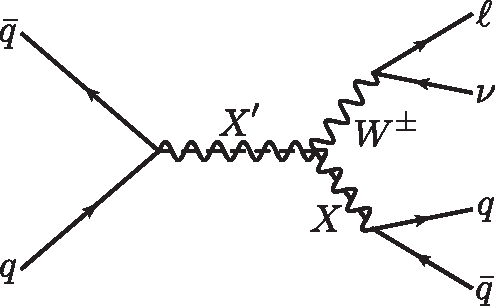
\includegraphics[width=0.48\columnwidth]{figs/2res.pdf}
}
\hspace{1.0cm}
\subfigure[t-channel]{
  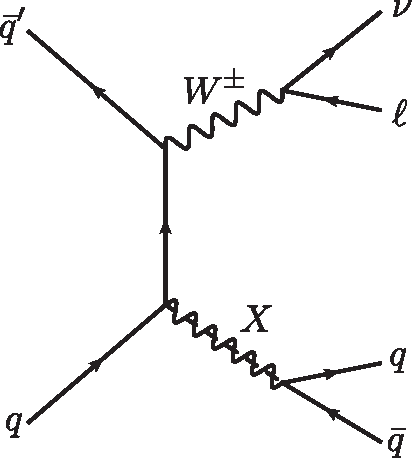
\includegraphics[width=0.33\columnwidth]{figs/1res.pdf}
}
  \caption{Representative Feynman diagrams for the 
    $s$-channel (left) and $t$-channel (right) topologies. 
    $X$ and $X'$ can be either a scalar or a vector boson. 
    \label{fig:resfeyn}} 
\end{figure}
%%%%%%%%%%%%%%%%
%%%%%%%%%%%%%%%%%%%%%%%%%%%%%%%%%%%%%%%%%%%%%%%
%%%%%%%%%%%%%%%%%%%%%%%%%%%%%%%%%%%%%%%%%%%%%%%
\subsection{How much LHC data are needed to observe/exclude CDF anomaly ?}
\label{sec:dataneeded}
Buckley \textit{et al}~\cite{BuckleyHooperMartin} 
performed a dedicated study to assess the 
ability of the ATLAS and CMS experiments at the LHC to 
probe the $\ell\nu+\text{dijet}$ channel in which the CDF 
anomaly was initially reported, as well as some additional channels.
They used the benchmark models outlined in Sec.~\ref{sec:models}, 
and calculated the expected cross section (before and after 
branching ratios and experimental cuts are applied) for each.
From this study they 
determine the required luminosity for each experiment to 
observe a $S/\sqrt{B} = 3$ deviation from the Standard Model prediction. 
In each case, they use an acceptance window of 60~GeV around 
the nominal center (150~GeV) of the mass peak in the dijet 
invariant mass and calculate $S/\sqrt{B}$ considering only 
statistical errors.
For all channels, the signal cross sections and the required luminosities 
are reported in Table~\ref{tab:LHC}.
%%%%%%%%%%%%%%%%%%%%
\begin{table}[ht]
  \begin{center}
  \renewcommand{\arraystretch}{1.2}
  \begin{tabular}{l|c|rrr@{\hspace{-0.6cm}}p{0.1cm}@{\hspace{1cm}}r}
    \hline \hline  
    & & $\ell\nu+jj$ & $\ell\ell+j j$ & $\nu \nu +j j$ && $\gamma + j j$ \\ 
    \hline
                   & $\sigma$ (fb)                                        & 11400 & 3400   & 3400 && 3450  \\
    Z' left-handed & $\sigma\times BR\times\cal{A}\times$ $\varepsilon$ (fb) &   145 &  13.7  &   99 &&   5.3 \\
                   & Required Lumi (fb$^{-1})$                            &   6.4 &  75    &  6.5 &&  170  \\
    \hline
                   & $\sigma$ (fb)                                        & 11400 & 3800   & 3800 && 6900   \\
    Z' universal   & $\sigma\times BR\times\cal{A}\times$ $\varepsilon$ (fb) &   143 &  14.4  &  106 &&   11.9 \\
                   & Required Lumi (fb$^{-1})$                            &   6.6 &  67    &  5.7 &&  34.4  \\
    \hline
                   & $\sigma$ (fb)                                        &  7970 & 2200   & 2200 && 1870   \\
    Technicolor    & $\sigma\times BR\times\cal{A}\times$ $\varepsilon$ (fb) &  188  &  18.8  &   75 &&   6.9  \\
                   & Required Lumi (fb$^{-1})$                            &   3.8 &  40    & 11.3 &&  103   \\
    \hline \hline  
  \end{tabular}
  \end{center}
  \caption{Cross sections (before and after branching ratios and
    experimental cuts) and the required luminosity for achieving a
    signal-to-square root background ratio ($S/\sqrt{B}$) of 3 at
    7~TeV for several new physics models. Reproduced from
    Ref.~\cite{BuckleyHooperMartin}.}
  \label{tab:LHC}
\end{table}
%%%%%%%%%%%%%%%%%%%%
%%%%%%%%%%%%%%%%%%%%%%%%%%%%%%%%%%%%%%%%%%%%%%%
\subsection{Previous experimental studies at LHC}
\label{sec:previousLHC}
Studies for $(W^\pm \to \ell \nu)+(\text{1--4})$ jets are available 
from ATLAS (using 1.3~pb$^{-1}$ of data) 
\cite{ATLASWVjets}, and the 
$(W^\pm \to \ell \nu) + n\text{ jets}$, 
$(Z\to\ell^+\ell^-)+n\text{ jets}$ final states have been 
studied at CMS (with 36~pb$^{-1}$ of data) \cite{CMSVjets}. 
A more recent study from ATLAS, presented at EPS \cite{ATLASWdijet}, 
used 1.02 fb$^{-1}$ of data and cuts modeled on CDF.
No direct evidence of the CDF anomaly has been found so far in any 
of these analyses.
Currently, about 5~fb$^{-1}$ of LHC data has been recorded and is
being analyzed. Many of the new physics 
scenarios proposed to explain the CDF excess should become 
visible at the LHC with $\sim5$~fb$^{-1}$ of data.
%%%%%%%%%%%%%%%%%%%%%%%%%%%%%%%%%%%%%%%%%%%%%%%
